% AUTO-GENERATED by writeup/make_rehaul_economics.py -- do not edit; re-run the script.
\begin{figure}[tbp]
\centering
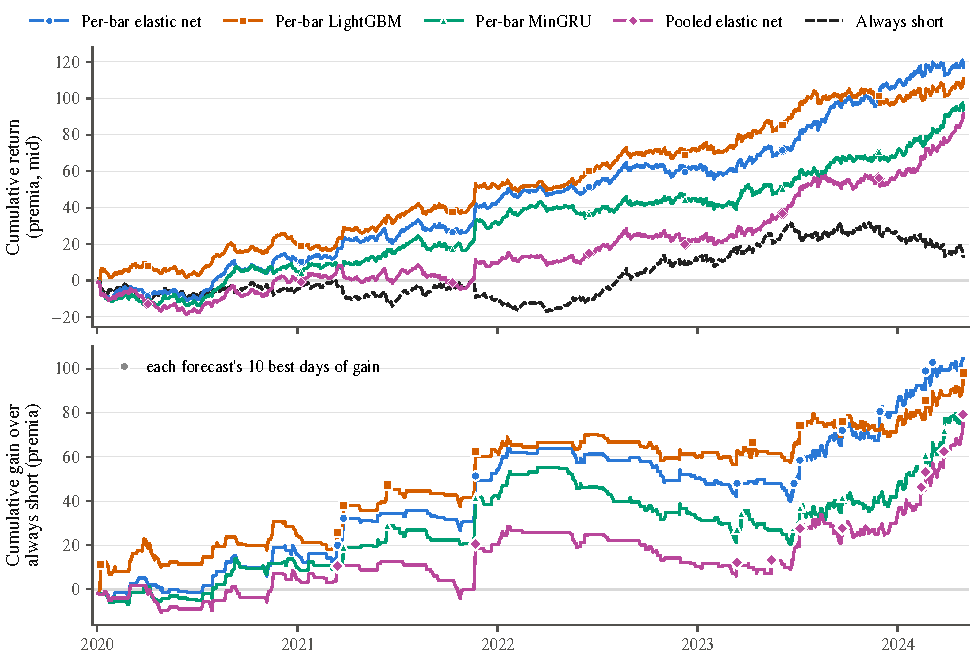
\includegraphics[width=\linewidth]{figures/rehaul_econ_cumpnl.pdf}
\caption{The closing trade over time, $q_t = \sign(s_t)$ at mid, for one forecast per family (all features) and
always short. Top: cumulative return $\sum_{u \le t} r_u$, in units of the straddle premium. Bottom: cumulative gain
over always short, $\sum_{u \le t} \bigl(r_u - r^{\mathrm{short}}_u\bigr)$; the markers are each forecast's 10
days of largest gain, each a day on which it bought and $R_t \ge 2.99$. The gain over the 866 days is
per-bar elastic net $+104.7$, per-bar LightGBM $+98.1$, per-bar MinGRU $+81.1$, pooled elastic net $+79.3$; without each forecast's 10 best days it is $+15.6$, $+2.4$, $-6.2$, $-6.3$. For 102 of the 112 forecasts of the model set the
gain is negative without their 10 best days.}
\label{fig:rh_econ_cumpnl}
\end{figure}
